% !TEX encoding = UTF-8 Unicode
% !TEX program = lualatex

\documentclass[twocolumn,10pt,a4j]{ltjsarticle}
\usepackage{kougai}

\title{カラーユニバーサルデザイン(CUD)の学習支援ツールの開発}
\author{2032116 永溝 柊介  指導教員 須田 宇宙 准教授}
\date{}

\begin{document}

\maketitle

\section{はじめに}

%背景1
遺伝子の異常により通常と色の見え方が異なる色覚を持つ色覚異常者は,男性で5%,女性で0.2%存在する\cite{okabe2003}.
色覚異常には,主に赤を感じづらいP型色覚,緑を感じづらいD型色覚,青を感じづらいT型色覚がある.
色覚の多様性に配慮し,より多くの人に伝わりやすいデザインとしてカラーユニバーサルデザイン(CUD)がある.

%背景2
学生や社会人になると,ゼミや業務等で資料を作成する機会が増加する.
そのため,CUDの講習では資料作成を実践し評価する機会が設けられている.
しかし,講習を受けた学生の20%がCUDに配慮していない資料を作成した\cite{sugamiya2020}.
先行研究では,講習内容を即座に理解することが困難なことが要因と考察されている.
そのため,CUDに配慮した工夫を一つ一つ実践する機会が必要だと考える.

%問題点2
学習者は別色覚での見え方を確認することでCUDをより理解できると考えられるが,現状では別媒体のシミュレータを使う必要がある.
また,評価者にとって学習者の作成物のCUD適合度を即座に判断することが難しく,評価や改善案を即座に提示することは困難である.
そのため,学習の際は,別色覚での見え方を即座に確認でき,自動で評価・改善案の提示を行う環境が望ましい.

%目的
そこで本研究では,これらの環境を持ち,CUDに配慮した工夫を項目ごとに実践できる学習ツールの開発を行う.
そして,開発した学習ツールを学習者が利用することでCUDに配慮した資料を作成できるか検証することを目的とする.

\section{色覚異常の見え方}
図\ref{fig:pcolor}はP型色覚での色の見え方を表している.
改善前は線1は緑色,線2は赤色であるが,P型色覚では区別が付きづらい.
対して,改善後では線2を橙色にし,点線にすることで区別が付きやすくした.
このように,色覚異常者にも正確に伝えるには,CUDに配慮する必要がある.

\begin{figure}[h]
\begin{center}
 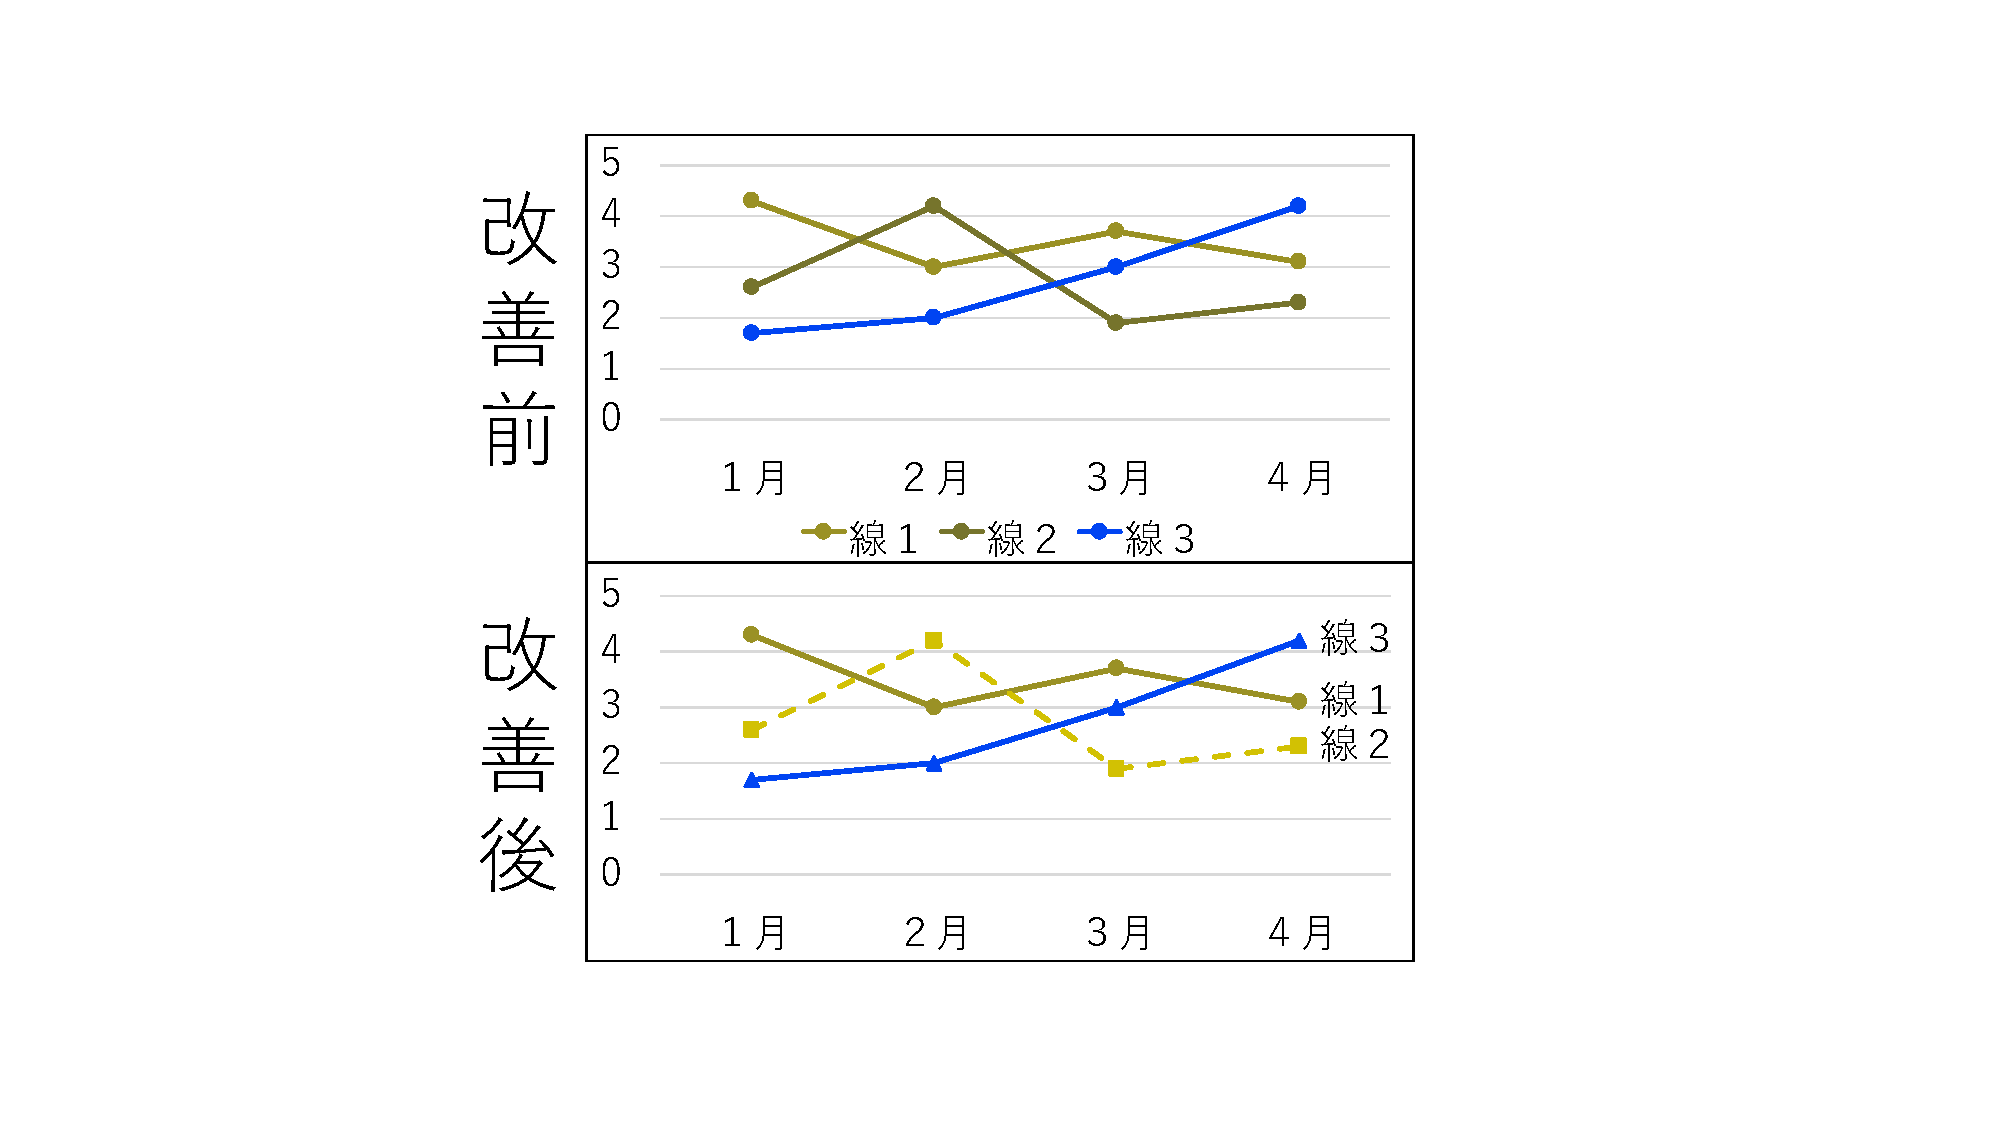
\includegraphics[clip,width=58mm,height=50mm]{images/pcolor.pdf}
\end{center}
 \caption{P型色覚者の見え方}
 \label{fig:pcolor}
\end{figure}

\section{実践内容}
%実践の概要
本研究では,開発した学習ツールを学習者が利用することでCUDに配慮した資料を作成できるか検証した.

%学習ツールの説明
本学習ツールは3部構成であり,1部で文字の強調,2部で色の組み合わせ,3部でグラフ作成での工夫を学習する.


例として文字の強調における配色を学ぶ項目の学習の流れを説明する.
選択肢から色を選択すると文の一部の色を変化させ,評価ボタンが押されると別色覚での見え方と評価・改善案を表示する.
そして,色を再選択もしくは次の項目に進む.
このように,CUDに配慮した工夫を項目ごとに実践できる学習ツールを開発した.

%実践内容
この学習ツールを用いて,学生10名を対象に検証した.
対象者には,東京都が作成したCUDのガイドラインを参考に色覚異常とCUDについて事前に説明した.
そして,対象者には学習ツールを利用した後に,Microsoft PowerPointを用いてスライドを作成してもらった.
そのスライドをCUDに配慮されているか項目別に評価した.
評価項目は,先行研究での評価項目に,アンダーライン等の装飾に関する項目を加えた5項目である.
項目ごとに,CUDに配慮した工夫が取り入れられていた資料の割合を図\ref{fig:result}に示す.

%結果
強調目的の配色でCUDに配慮された資料は90%であり,先行研究に比べて10ポイント増加している.
また,色の組み合わせでは,全ての資料がCUDに配慮した配色となっていた.

\begin{figure}[h]
\begin{center}
 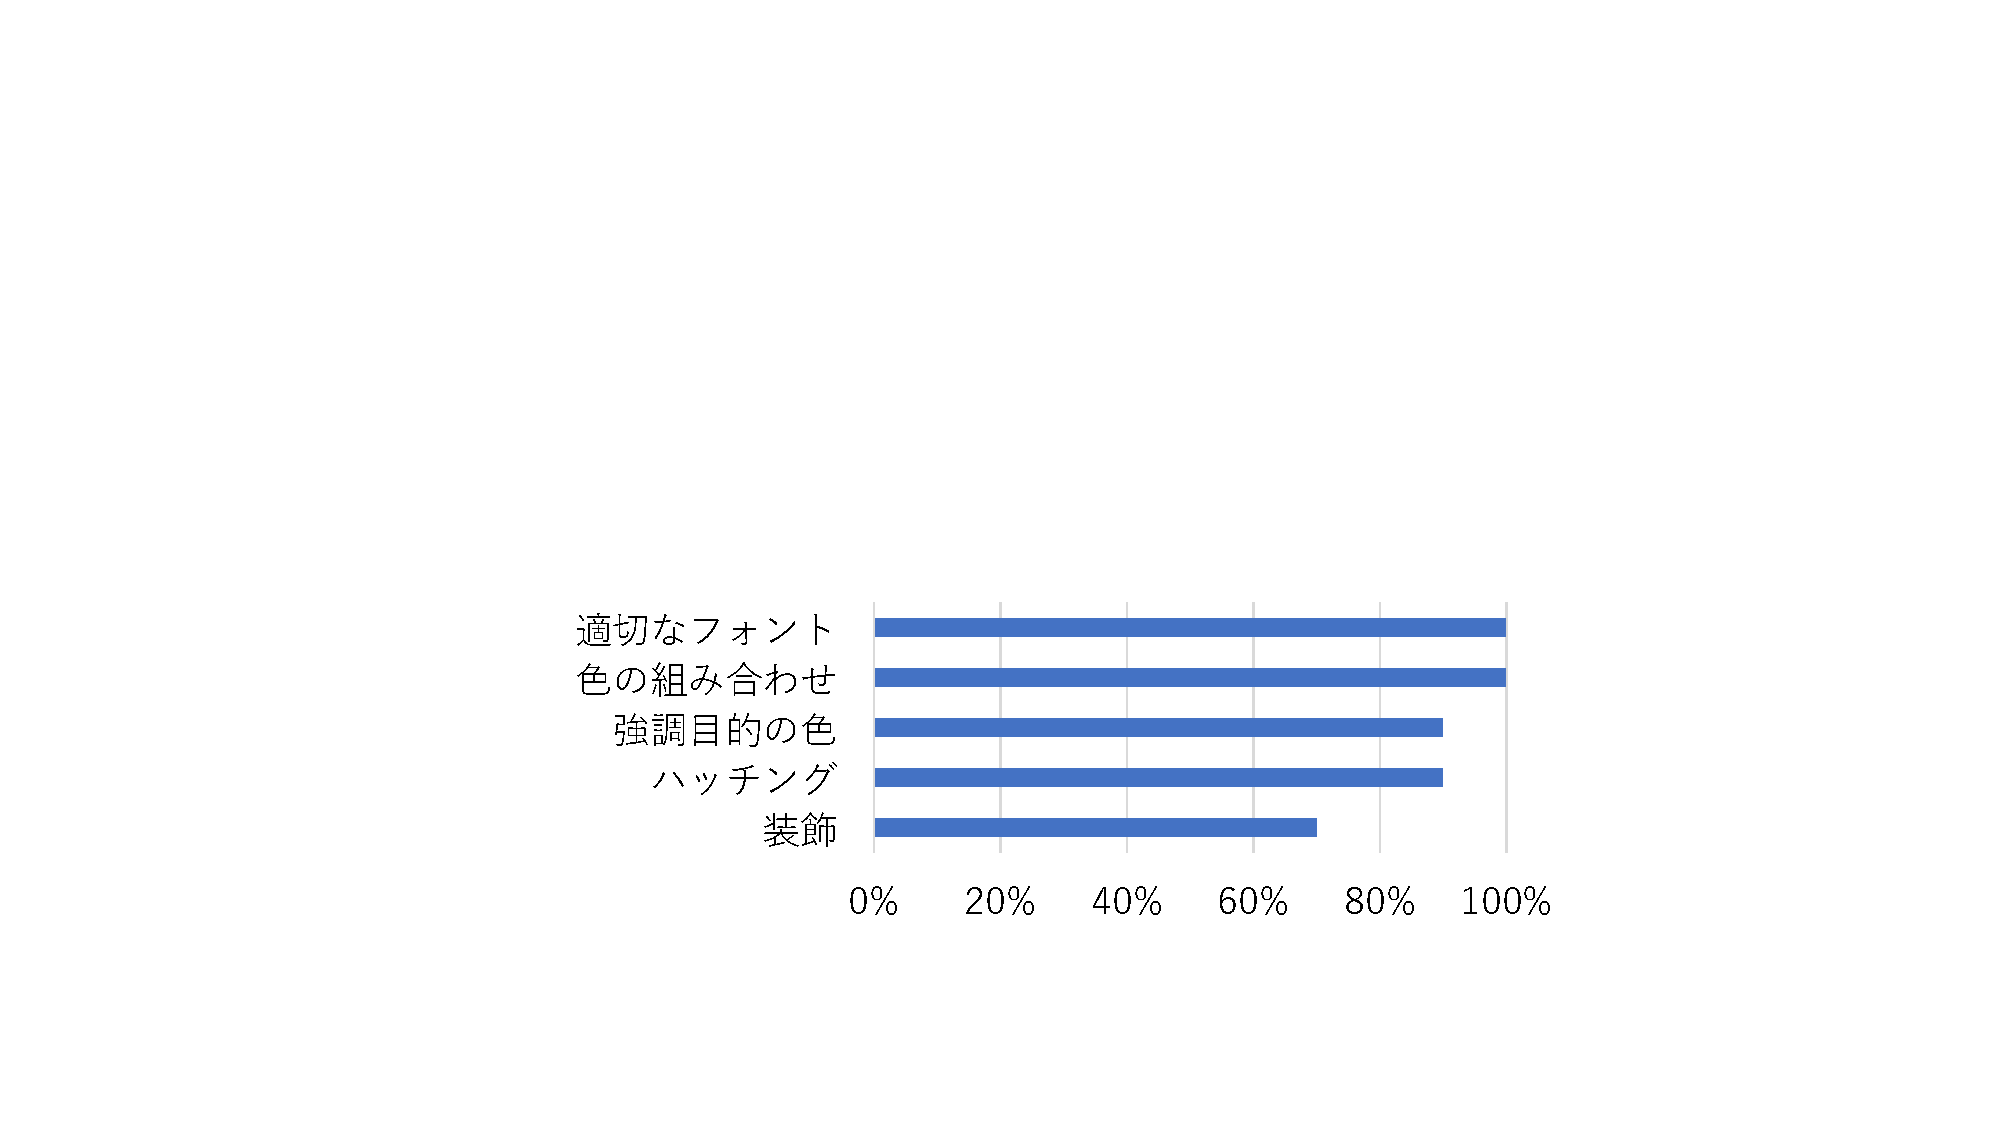
\includegraphics[clip,width=72mm,height=24mm]{images/result.pdf}
\end{center}
 \caption{スライドのCUD評価結果}
 \label{fig:result}
\end{figure}



\section{おわりに}
本研究では,学習者がCUDに配慮した工夫を項目ごとに実践できる学習ツールを開発した.
開発した学習ツールを学習者が利用することで,CUDに配慮した資料を作成できるという結果が得られた.
一方,他項目に比べて工夫が行われていない項目があるため,学習の流れや表示項目等の改善が望まれる.




\begin{thebibliography}{99}
\bibitem{okabe2003}岡部正隆・伊藤啓・橋本知子: ``ユニバーサルデザインにおける色覚バリアフリーへの提言'', \url{https://www.nig.ac.jp/color/handout1.pdf}, 2023/7/3参照

\bibitem{sugamiya2020} 菅宮恵子: ``色覚異常を考慮した教材資料作成実習の実践報告とその評価'', 教職・学芸員課程研究,2号(2020),p.14-23, 2023/7/3参照
\end{thebibliography}

\end{document}
